\documentclass[a4paper,12pt]{article}


\usepackage[MeX]{polski}
\usepackage[utf8]{inputenc}	% kodowanie znaków
\usepackage{indentfirst}

\usepackage{upquote}  	% zamiana cudzysłowów klasycznych (,, ") na górne (" ") w kodach źródłowych
\usepackage{graphicx}	% wstawianie obrazków
\usepackage{amsmath}
\usepackage{listings}


\def\PICSDIR{PICS}

% Ustawienie marginesów
\oddsidemargin=0.5cm
\evensidemargin=-0.5cm
\topmargin=0cm
\textwidth=16cm
\textheight=23cm

% Ładniejsze tabelki
\usepackage{booktabs}


\frenchspacing

\clubpenalty=10000		% to kara za sierotki
\widowpenalty=10000		% nie pozostawia wdów
\brokenpenalty=10000 	% nie dzieli wyrazów pomiędzy stronami


\sloppy

% Pakiety z ładnymi czcionkami
\usepackage[T1]{fontenc}
\usepackage{lmodern}


% Ładniejsze tabelki
\usepackage{booktabs}

% Ustawienia wyglądu listingów
\lstset{
	language=C++,                               % choose the default language of the code
	basicstyle=\footnotesize\ttfamily,       	% the size of the fonts that are used for the code
	numbers=left,                   		% where to put the line-numbers
%	numberstyle=\tiny,      			% the size of the fonts that are used for the line-numbers
	stepnumber=1,                   		% the step between two line-numbers. If it's 1 each line will be numbered
	numbersep=5pt,                  		% how far the line-numbers are from the code
	showspaces=false,               		% show spaces adding particular underscores
	showstringspaces=false,         	% underline spaces within strings
	showtabs=false,                 		% show tabs within strings adding particular underscores
	tabsize=4,	                		% sets default tabsize
	captionpos=b,                   		% sets the caption-position
	breaklines=true,                		% sets automatic line breaking
	breakatwhitespace=true,        	% sets if automatic breaks should only happen at whitespace
	extendedchars=true,
	keywordstyle=\bfseries,
	identifierstyle=,
	commentstyle=\slshape,
	stringstyle=\slshape,
	xleftmargin=30pt,
	frame=tb,
	framexleftmargin=30pt,
}

\begin{document}

\title{{\small Programowanie równoległe i rozproszone}\\Algorytm szyfrujący AES w trybie CTR}
\author{Maciej Stefańczyk, Kacper Szkudlarek}

\maketitle

\begin{abstract}
Dokumentacja realizacji projektu z przedmiotu "Programowanie równoległe i rozproszone". W ramach projektu wykonana została implementacja algorytmu szyfrującego AES (Advanced Encryption Standard) pracującego w trybie CTR (Counter mode). Zrównoleglenie zostało oparte o bibliotekę OpenMP dla pamięci wspólnej, oraz MPI dla pamięci rozproszonej.
\end{abstract}


\section{Wstęp}
Algorytm szyfrujący AES (ang. Advanced Encryption Standard) jest to symetryczny szyfr blokowy przyjęty przez NIST (ang. National Institute of Standards and Technology) jako standard szyfrowania. Algorytm został stworzony w ramach ogłoszonego konkursu, który miał wyłonić następcę algorytmu DES(ang. Data Encryption Standard). Jego robocza nazwa to Rijndael. Ze względu na swą złożoność algorytm uważany jest za bezpieczny i powszechnie stosowany. 

Algorytm szyfruje i deszyfruje dane w 128-bitowych blokach, korzystając z 128, 192 lub 256 bitowych kluczy. Dane, na których operuje algorytm formowane są w macierz 4x4, w której każda komórka jest jednym bajtem danych. W zależności do wybranej wielkości klucza szyfrującego wykonywane jest odpowiednio 10, 12 lub 14 rund szyfrujących. Wszystkie rundy poza pierwszą i ostatnią składają się z czterech kroków:
\begin{enumerate}
\item Etap: substytucja wstępna  - jest to nielinowe przekształcenie każdego bajtu poprzez zamianę jego wartości zgodnie z tablicą LUT.
\item Etap: zamiana wierszy - na każdym wierszu danych wykonywana jest operacja rotacji cyklicznej o zadaną liczbę pozycji.
\item Etap: mieszanie kolumn - każda kolumna poddawana jest odwracalnej liniowej transformacji.
\item Etap: dodanie klucza rundowego - do danych dodawany jest klucz rundowy wygenerowany na podstawie klucza głównego.
\end{enumerate}

W opisywanej implementacji algorytm szyfrowania AES pracował w trybie CTR (ang . Counter). Jest to tzw. tryb licznikowy. Pozwala wykorzystać on szyfry blokowe do kodowania m.in. strumieni danych. Generowany jest pseudolosowy ciąg danych, który który pełni rolę strumienia szyfrującego. Jest on mieszany poprzez użycie operacji XOR z danymi wejściowymi, przez co uzyskujemy zaszyfrowany ciąg danych. Zostało to przedstawione na rysunku (\ref{rys:ctr}).

\begin{figure}
\centering
\includegraphics[width=\textwidth]{\PICSDIR/CTR_mode.pdf}
\caption{Schemat działania trybu licznikowego.}
\label{rys:ctr}
\end{figure}

\section{Implementacja}
W ramach projektu powstały trzy wersje oprogramowania opisane w dalszych paragrafach:
\begin{enumerate}
\item Wersja sekwencyjna - jest to implementacja algorytmu w języku C wykonująca się jednowątkowo w sposób sekwencyjny.
\item Wersja wykorzystująca pamięć współdzieloną - jest to rozwinięcie wersji sekwencyjnej, które dzięki wykorzystaniu OpenMP pozwala na równoległe wykonywanie na wielu procesorach.
\item Wersja wykorzystująca pamięć rozproszoną - jest to rozwinięcie wersji sekwencyjnej, które dzięki wykorzystaniu protokołu MPI pozwala na równoległe wykonywanie na wielu maszynach połączonych między sobą siecią.
\end{enumerate}



\subsection{Wersja sekwencyjna}

Diagram przepływu danych dla stworzonej aplikacji został przedstawiony na rysunku (\ref{rys:da}).  Na podstawie danych podanych w wierszu poleceń w czasie wykonywania programu podejmowane są decyzje o trybie działania - szyfrowanie, deszyfrowanie, długości wykorzystanego klucza, pobierane są dane wejściowe.

Dane podawane do programu (klucz, dane do szyfrowania/deszyfrowania) odczytywane są bezpośrednio z plików i wczytywane w całości do pamięci. Dzięki takiemu rozwiązaniu narzut czasowy związany z odczytem i zapisem danych w czasie ich szyfrowania jest stosunkowo niewielki, gdyż wszystkie operacje przeprowadzane są na pamięci, a nie na plikach dyskowych. Powoduje to jednak wydłużenie czasu wczytywania danych, zwłaszcza przy dużych zbiorach, które maja być zaszyfrowane.

Pseudolosowa liczba wykorzystywana w trybie CTR do szyfrowania strumienia danych została zaimplementowana w postaci złożenia czterech 32 bitowych bloków. Najbardziej znaczące 32 bit wypełniane jest wartością czasu odczytaną w momencie ładowania do pamięci pliku z danymi do zaszyfrowania. Kolejne dwa bloki 32 bitowe stanowią liczby odpowiednio 1 i 0. Do najmniej znaczących 32 bit wpisywana jest wartość licznika zliczającego ilość zaszyfrowanych bloków. W czasie zapisywania wyników wartość górnych 64 bitów zapisywana jest na samym początku pliku wynikowego.

Wykorzystane w środkowej części liczy pseudolosowej wartości 1 i 0 w celu zwiększenia bezpieczeństwa należałoby zastąpić jakimiś bardziej skomplikowanymi wartościami.

W celu optymalizacji przetwarzania danych zostały wprowadzone pewne modyfikacje w sposobie przechowywania i zapisywania macierzy stanu algorytmu. Każda kolumna przechowywana jest w pamięci w postaci 32 bitowej liczby. Takie potraktowanie kolumn pozwoliło znacząco ułatwić proces "mieszania" kolumn w trakcie szyfrowania.

\begin{figure}
\centering
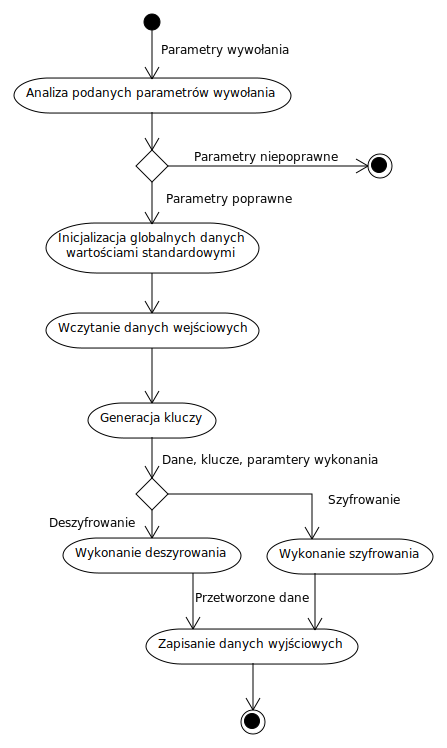
\includegraphics[width=\textwidth, height=0.95\textheight]{\PICSDIR/diagram_aktywnosci.pdf}
\caption{Diagram przepływu danych w czasie wywołanie programu.}
\label{rys:da}
\end{figure}

\subsection{Pamięć wspólna -- OpenMP}
\textbf{OpenMP} (ang. Open Multi-Processing)  jest to wieloplatformowy interfejs programowania aplikacji umożliwiający tworzenie aplikacji dla systemów wieloprocesorowych korzystających z pamięci współdzielonej. Interfejs może być wykorzystywany w językach C, C++ i FORTRAN, na architekturach Unix i Windows. Do sterowania sposobem wykonywania programu używa się zbiory dyrektyw kompilatora oraz zmiennych środowiskowych.

Dzięki zastosowaniu trybu licznikowego (CTR) w implementacji algorytmu AES możliwe było bardzo dobre zrównoleglenie przeprowadzanych obliczeń. W tym trybie każdy 128 bitowy blok danych szyfrowany jest niezależnie od pozostałych. Jedynym elementem, który należy kontrolować jest takie modyfikowanie licznika, by możliwe było późniejsze odtworzenie jego pracy w celu odszyfrowania danych.

W celu oznaczenia bloku do zrównoważenia użyta została następująca dyrektywa: \\
 \texttt{\#pragma omp parallel for default(none) private(i) shared(data, in\_blocks, in\_ptr32)}\\
Odnosząca się do następującego bolku kodu:\\
\begin{lstlisting}
	for (i = 0; i < in_blocks; ++i)
	{
		aes_state_t ctr = aesCipherCounter(data, i);
		uint32_t c0 = *(uint32_t*)ctr.s;
		uint32_t c1 = *(uint32_t*)ctr.s+4;
		uint32_t c2 = *(uint32_t*)ctr.s+8;
		uint32_t c3 = *(uint32_t*)ctr.s+12;
		in_ptr32[4 * i    ] = in_ptr32[4 * i    ] ^ c0;
		in_ptr32[4 * i + 1] = in_ptr32[4 * i + 1] ^ c1;
		in_ptr32[4 * i + 2] = in_ptr32[4 * i + 2] ^ c2;
		in_ptr32[4 * i + 3] = in_ptr32[4 * i + 3] ^ c3;
	}
\end{lstlisting}

Dyrektywa ta definiuje prywatne i współdzielone zmienne zawarte w wyróżnionym fragmencie. Jako prywatna została oznaczona zmienna sterująca pętla \texttt{for}, tak by każdy wątek mógł niezależnie przetwarzać dane. Zmiennymi publicznymi są natomiast:
\begin{itemize}
\item \texttt{data} - struktura danych zawierająca zmienne globalne,
\item \texttt{in\_blocks} - liczba bloków, które należy przetworzyć,
\item \texttt{un\_ptr32} - wskaźnik na przetwarzane dane.
\end{itemize}

Zrównoleglona pętla  \texttt{for} odpowiada za szyfrowanie algorytmem AES kolejnych chwilowych zmiennych losowych i przeprowadzanie operacji XOR tych zmiennych z szyfrowanymi danymi, a także operację odwrotną - deszyfrowanie. Tak przetworzone dane są przekazywane do zapisania w pliku wynikowym. 

\subsection{Pamięć rozproszona -- MPI}
\textbf{MPI} (ang. Message Passing Interface) jest to protokół komunikacyjny będący standardem przesyłania komunikatów w rzeczywistych i wirtualnych maszynach równoległych z pamięcią lokalną. 

Przy użyciu MPI powstała wersja oprogramowania umożliwiająca zrównoleglenie obliczeń  w oparciu o klaster.  Każdy z komputerów wchodzących w skład klastra dostaje porcję danych, którą przetwarza a następnie zawraca wyniki do procesu nadzorującego.

Najpierw tworzony jest komunikator. Wykorzystywany jest komunikator \texttt{MPI\_COMM\_WORLD} obejmujący wszystkie procesy, które mogą między sobą wymieniać dane. Odczytywana jest ilość komputerów w komunikatorze i dla każdego procesu jego id w tym komunikatorze. Następnie następuje przetworzenie danych, co zostało przedstawione na listingu.

\begin{lstlisting}
    // broadcast global data to all processes
    MPI_Bcast(&key_size, 1, MPI_INT, root, MPI_COMM_WORLD);
    MPI_Bcast(&direction, 1, MPI_INT, root, MPI_COMM_WORLD);
    MPI_Bcast(genkey, key_size/8, MPI_BYTE, root, MPI_COMM_WORLD);
    MPI_Bcast(&data.in_blocks, 4, MPI_BYTE, root, MPI_COMM_WORLD);
    MPI_Bcast(&data.nonce_0, 4, MPI_BYTE, root, MPI_COMM_WORLD);
    MPI_Bcast(&data.nonce_1, 4, MPI_BYTE, root, MPI_COMM_WORLD);

	aesInitGlobalData(&data, key_size);

    // allocate data buffer for each process
    data.in_data = malloc(data.in_blocks * data.block_size);
    aesKeyExpansion(&data, genkey);


    // scatter data to all processes
	MPI_Scatter(input_buffer, data.in_blocks*data.block_size, MPI_BYTE, data.in_data,  data.in_blocks*data.block_size, MPI_BYTE, root, MPI_COMM_WORLD);

	// process data - cipher/decipher given block
	aesCipherT(&data);

	// return processed data
	MPI_Gather(data.in_data, data.in_blocks*data.block_size, MPI_BYTE, input_buffer,  data.in_blocks*data.block_size, MPI_BYTE, root, MPI_COMM_WORLD);
\end{lstlisting}

Do każdego procesu wysyłane są zmienne globalne jak wielkość używanego klucza, klucz, kierunek pracy (szyfrowanie/deszyfrowanie danych), ilość wszystkich bloków do przetworzenia, a także wygenerowana wartość używana w czasie tworzenia zmiennej tymczasowej.
Następnie każdy z procesów alokuje sobie pamięć dla danych, które będzie przetwarzał. Przy użyciu funkcji \texttt{MPI\_Scatter} dane wejściowe aplikacji zostają podzielone i rozesłane do poszczególnych procesów, gdzie następuje ich przetworzenie jak w wersji sekwencyjnej. Po zakończeniu przetwarzania wszystkie procesy odsyłają dane a proces nadrzędny przy pomocy funkcji \texttt{MPI\_Gather} odbiera je i scala. Przetworzone dane wysyłane są do pliku wynikowego.


\subsection{Dodatkowe możliwości}

\subsection{Obsługa programu}

\section{Testy}

\subsection{Testy jednostkowe}

Testy jednostkowe mają za zadanie wykazanie poprawności działania poszczególnych elementów składowych tworzonego oprogramowania.  Dla opisywanej aplikacji powstały następujące testy:
\begin{enumerate}
\item \textbf{\texttt{test\_key}} - jest to test badający poprawność generowanych kluczu rundowych. Do funkcji podawane są dane testowe w postaci klucza pierwotnego, rozmiaru klucza, a także oczekiwanego wyniku. Funkcja testuje poprawność wygenerowanego klucza porównując go z podanym oczekiwanym wynikiem. 
\item \textbf{\texttt{test\_mix}} - jest to funkcja mieszanie kolumn macierzy stanu algorytmu szyfrującego. Pobiera dwa argumenty, pierwszym jest przykładowa macierz stanu, drugim oczekiwane rezultaty. Po wykonaniu operacji mieszania otrzymane wyniki porównywane są z otrzymanymi danymi.
\item \textbf{\texttt{test\_shift}} - jest to funkcja testująca poprawność operacji rotacji wierszy macierzy stanu algorytmu. Podobnie jak funkcja \texttt{test\_mix} pobiera dwa argumenty - przykładową macierz stanu i oczekiwany wynik operacji, z którym porównywane są otrzymane wyniki.
\item \textbf{\texttt{test\_ctr}} - jest to test badający poprawność szyfrowania zaimplementowanego algorytmu. Jako dane wejściowe pobierane są wektor inicjujący, dane do zaszyfrowania, oczekiwane wyniki oraz klucz, który ma być użyty do szyfrowania. Wektor użyty w tym teście jednostkowym został pobrany z publikacji NIST "Recommendation for Block Cipher Modes of Operation".
\end{enumerate}

\subsection{Testy wydajności}

Drugim wykonanym rodzajem testów stworzonej aplikacji są testy wydajnościowe. Zadanie testów było zmierzenie różnic w czasie wykonania tego samego zadania testowego przez różne wersje oprogramowania. Wyniki testów jednoznacznie pokazały wzrost wydajności aplikacji poprzez użycie narzędzi do zrównoleglania obliczeń.

\subsubsection{Dane testowe}

Do testowania stworzonych aplikacji przygotowany został zbiór danych testowych. Miał on postać pliku zawierającego pseudolosowe wygenerowane przy pomocy systemowego generatora liczb pseudolosowych sytemu Linux. Rozmiar danych wygenerowanych danych testowych to 10 MB.\\
\texttt{dd if=/dev/urandom of=pliktestowy count=10M}



\subsubsection{Wyniki}
Na rysunku \ref{rys:res_omp} przedstawione zostały cztery wykresy:
\begin{enumerate}
\item Zależności czasu przetwarzania części równoległej programu od ilości wątków przetwarzających.
\item Zależności czasu przetwarzania części sekwencyjnej programu od ilości wątków przetwarzających.
\item Współczynnik przyspieszenia przetwarzania danych równoległych w zależności od liczby wątków.
\item Współczynnik przyspieszenia programu w zależności od liczby wątków.
\end{enumerate}

Wyniki prezentowane na wykresach są zgodne z naszymi oczekiwaniami. Widać wyraźną zależność czasu przetwarzani danych od liczby wątków przetwarzających. Podobnie jest z wykresem współczynnika przyspieszenia. Obliczenia zostały wykonana na 4-rdzeniowej maszynie firmy SUN, z parametrem wykonania mówiącym o wykorzystaniu 16 wątków obliczeniowych.

Maksymalne przyspieszenie możemy obliczyć ze wzoru Amdahla:\\
$S(n,p)\overrightarrow{p \rightarrow \infty } \frac{1}{\beta(n, 1)} = $, \\
gdzie $S(n,p)$ to przyspieszenie, $\beta(n, 1)$ to czas wykonania części sekwencyjnej na maszynie z $p$ procesorami.

\begin{figure}
\centering
\includegraphics[width=\textwidth]{\PICSDIR/threads.pdf}
\caption{Wyniki testów wydajnościowych aplikacji zrównoleglonej przy użyciu OpenMP.}
\label{rys:res_omp}
\end{figure}



\begin{table}[h!]
\caption[Zadanie pierwsze -- czas przetwarzania pojedynczej ramki obrazu]{Czas przetwarzania pojedynczej ramki obrazu}
\centering
\begin{tabular}{lcccccccc}
\toprule
 & \multicolumn{2}{c}{1280x720} & \multicolumn{2}{c}{960x540} & \multicolumn{2}{c}{640x360} & \multicolumn{2}{c}{320x180} \\
\cmidrule(r){2-9}
 & czas [ms] & FPS & czas [ms] & FPS & czas [ms] & FPS & czas [ms] & FPS \\
\midrule
FraDIA & \bf 45,7 & 21,9 & \bf 26,8 & 37,3 & \bf 12,7 & 78,7 & \bf 4,5 & 222,2 \\
RAW    & \bf 44,5 & 22,5 & \bf 26,1 & 38,3 & \bf 12,1 & 82,6 & \bf 4,3 & 232,6 \\
\bottomrule
\end{tabular}
\label{tab:zad_1_wyniki}
\end{table}

\end{document}
